\documentclass[UTF8]{ctexart}

\usepackage{amsmath,amssymb,graphicx,geometry}

\geometry{margin=25mm}

\title{CMC-Bench 题目册}

\date{2026年11月10日}

\begin{document}

\maketitle

难度为未校准的初步结构标签。本册仅含题目，不含解答。

\section*{CMC-2009-PRE-Math-I — 圆柱面 / 正交投影}

dev，L4。

求经过三条平行直线 $L_1:x=y=z$，$L_2:x-1=y=z+1$，$L_3:x=y+1=z-1$ 的圆柱面方程。

\section*{CMC-2009-PRE-Math-II — 伴随矩阵 / 交换子 / 循环向量}

dev，L6。

设 $F$ 为首一多项式 $x^n+a_1x^{n-1}+\cdots+a_n$ 的伴随矩阵：次对角线为1，末列为 $(-a_n,\ldots,-a_1)^T$，其余为0。若 $A=(b_{ij})\in\mathbb C^{n\times n}$ 且 $AF=FA$，证明 $A=\sum_{j=1}^n b_{j1}F^{j-1}$；求子空间 $\{X:FX=XF\}$ 的维数。

\section*{CMC-2009-PRE-Math-III — 交换关系 / 迹 / 公共特征向量}

dev，L6。

设 $V$ 为n维复线性空间，$n>0$，线性变换 $f,g$ 满足 $fg-gf=f$。证明f的特征值全为0，且f,g有公共特征向量。

\section*{CMC-2009-PRE-Math-IV — 等度连续 / 一致收敛 / 可导性}

dev，L5。

设无穷次可微函数列 $f_n:[a,b]\to\mathbb R$ 逐点收敛，且统一满足 $|f_n^{\prime}(x)|\le M$。(1) 证明一致收敛；(2) 极限函数是否必处处可导？说明理由。

\section*{CMC-2009-PRE-Math-V — 三角积分 / 级数比较}

dev，L6。

令 $a_n=\int_0^{\pi/2}t\left|\frac{\sin nt}{\sin t}\right|^3dt$。证明 $\sum_{n=1}^\infty1/a_n$ 发散。

\section*{CMC-2009-PRE-Math-VI — Laplace算子 / 极坐标 / 径向积分}

dev，L5。

设f在闭单位圆盘上二次连续可微，满足 $f_{xx}+f_{yy}=x^2y^2$。求 $\iint_{x^2+y^2\le1}\frac{xf_x+yf_y}{\sqrt{x^2+y^2}}dxdy$。

\section*{CMC-2009-PRE-Math-VII — Rolle定理 / 弦线}

dev，L2。

f在[0,1]连续、在(0,1)二阶可导，端点连线与曲线还有内点 $(c,f(c))$，$0<c<1$。证明存在 $\xi\in(0,1)$ 使 $f^{\prime\prime}(\xi)=0$。

\section*{CMC-2009-FINAL-NonMath-I-1 — 一致Taylor估计 / 求和极限}

dev，L3。

求 $\lim_{n\to\infty}\sum_{k=1}^{n-1}(1+k/n)\sin(k\pi/n^2)$。

\section*{CMC-2009-FINAL-NonMath-I-3 — 约束最优化 / 圆柱体}

dev，L2。

设计容积V的封闭圆柱容器，上下底每单位面积材料费a，侧面每单位面积材料费b，a,b>0。高度与底面直径之比为何值时总费用最小？

\section*{CMC-2009-FINAL-NonMath-I-4 — 三角有理积分 / 换元}

dev，L4。

f′(x)=1/(sin³x+cos³x)，1/4<x<1/2，求f(x)。

\section*{CMC-2009-FINAL-NonMath-II-1 — 指数极限 / 二阶展开}

dev，L2。

求 $\lim_{n\to\infty}n[(1+1/n)^n-e]$。

\section*{CMC-2009-FINAL-NonMath-II-2 — 幂平均 / 指数极限}

dev，L2。

a,b,c>0，求 $\lim_{n\to\infty}[(a^{1/n}+b^{1/n}+c^{1/n})/3]^n$。

\section*{CMC-2009-FINAL-NonMath-III — 导数定义 / 复合极限}

dev，L2。

f在1邻域有定义且在1可导，f(1)=0、f′(1)=2。求 $\lim_{x\to0}f(\sin^2x+\cos x)/(x^2+x\tan x)$。

\section*{CMC-2009-FINAL-NonMath-IV — 反常积分 / Cesàro极限}

dev，L4。

f在[0,∞)连续且∫₀∞f收敛。求 $\lim_{y\to\infty}\frac1y\int_0^yxf(x)dx$。

\section*{CMC-2009-FINAL-NonMath-V — 中值定理 / 辅助函数}

dev，L4。

f在[0,1]连续、(0,1)可导，f(0)=f(1)=0、f(1/2)=1。(1)证明存在ξ∈(1/2,1)使f(ξ)=ξ；(2)证明存在η∈(0,ξ)使f′(η)=f(η)-η+1。

\section*{CMC-2009-FINAL-NonMath-VI — 截断指数 / 积分中值}

dev，L5。

n>1为整数，$F(x)=\int_0^xe^{-t}\sum_{k=0}^nt^k/k!\,dt$。证明F(x)=n/2在(n/2,n)内至少有一个根。

\section*{CMC-2009-FINAL-NonMath-VII — 函数迭代 / 导数 / 不动点}

dev，L6。

是否存在R上的可微函数f，使f(f(x))=1+x²+x⁴-x³-x⁵？若存在请举例，否则证明不存在。

\section*{CMC-2009-FINAL-NonMath-VIII — 一致连续 / 等度连续}

dev，L4。

f在[0,∞)一致连续，对每个固定x≥0有f(x+n)→0。证明函数列f(x+n)在[0,1]上一致收敛到0。

\section*{CMC-2009-PRE-NonMath-I-1 — 二重积分 / 变量代换}

dev，L3。

设D为x≥0,y≥0,x+y≤1。计算 $\iint_D\frac{(x+y)\ln(1+y/x)}{\sqrt{1-x-y}}dxdy$。

\section*{CMC-2009-PRE-NonMath-I-2 — 函数方程 / 定积分}

dev，L1。

连续函数f满足 $f(x)=3x^2-\int_0^2f(t)dt-2$，求f。

\section*{CMC-2009-PRE-NonMath-I-3 — 切平面 / 法向量}

dev，L2。

求曲面 $z=x^2/2+y^2-2$ 上与 $2x+2y-z=0$ 平行的切平面。

\section*{CMC-2009-PRE-NonMath-I-4 — 隐函数 / 二阶导数}

dev，L3。

设 $xe^{f(y)}=e^y\ln29$ 确定y=y(x)，f有二阶导且f′(y)≠1。求y″。

\section*{CMC-2009-PRE-NonMath-II — 幂指极限 / Taylor展开}

dev，L2。

给定正整数n，求 $\lim_{x\to0}[(e^x+e^{2x}+\cdots+e^{nx})/n]^{e/x}$。

\section*{CMC-2009-PRE-NonMath-III — 含参积分 / 导数连续性}

dev，L3。

f连续，$g(x)=\int_0^1f(xt)dt$，且f(x)/x→A当x→0。求g′，讨论g′在0处的连续性。

\section*{CMC-2009-PRE-NonMath-IV — Green公式 / 积分不等式}

dev，L4。

L为正方形[0,π]²的正向边界。证明 $\oint_Lxe^{\sin y}dy-ye^{-\sin x}dx=\oint_Lxe^{-\sin y}dy-ye^{\sin x}dx$，并证明该值≥5π²/2。

\section*{CMC-2009-PRE-NonMath-V — 线性方程 / 解之差}

dev，L3。

某二阶常系数非齐次线性微分方程有三个解 $xe^x+e^{2x}$、$xe^x+e^{-x}$、$xe^x+e^{2x}-e^{-x}$，求方程。

\section*{CMC-2009-PRE-NonMath-VI — 旋转体 / 约束极值}

dev，L4。

抛物线y=ax²+bx+2ln c过原点，在[0,1]上非负，且其下方与x轴、x=1围成面积1/3。确定a,b,c使绕x轴旋转体积最小，并求最小体积。

\section*{CMC-2009-PRE-NonMath-VII — 微分方程 / 函数项级数}

dev，L4。

对正整数n，$u_n^{\prime}(x)=u_n(x)+x^{n-1}e^x$，$u_n(1)=e/n$。求 $\sum_{n=1}^\infty u_n(x)$ 的收敛区间与和。

\section*{CMC-2009-PRE-NonMath-VIII — Riemann和 / 奇异极限}

dev，L5。

当x→1−时，求与 $\sum_{n=0}^\infty x^{n^2}$ 等价的无穷大量。

\section*{CMC-2010-FINAL-Math-I — 椭球 / 中心圆截面}

dev，L5。

求所有过原点且截椭球4x²+5y²+6z²=1为圆的平面。

\section*{CMC-2010-FINAL-Math-II — 矩积分 / 重排不等式}

dev，L5。

0<f(x)<1，∫₀∞f和∫₀∞xf均收敛。证明 $\int_0^\infty xf(x)dx>\tfrac12(\int_0^\infty f(x)dx)^2$。

\section*{CMC-2010-FINAL-Math-III — Abel求和 / 级数尾项}

dev，L5。

若∑ₙ₌₁∞naₙ收敛，令 $t_n=\sum_{k=1}^\infty ka_{n+k}$。证明tₙ定义良好且tₙ→0。

\section*{CMC-2010-FINAL-Math-IV — 交换子算子 / 对角化}

dev，L4。

A∈Mₙ(C)，$σ_A$(X)=AX-XA。证明A可对角化时$σ_A$也可对角化。

\section*{CMC-2010-FINAL-Math-V — 近似可加 / 函数稳定性}

dev，L7。

连续f:R→R满足$sup_{x,y∈R}$|f(x+y)-f(x)-f(y)|<∞。证明存在a∈R使supₓ|f(x)-ax|<∞。

\section*{CMC-2010-FINAL-Math-VI — 迹泛函 / 对偶基 / 双线性型}

dev，L7。

非零线性映射φ:Mₙ(R)→R满足φ(XY)=φ(YX)。定义(X,Y)=φ(XY)。(1)证明此型非退化；(2)任取基A₁,…,Aₙ²及其对此型的对偶基B₁,…,Bₙ²，证明∑AᵢBᵢ为数量矩阵。

\section*{CMC-2010-PRE-Math-I — 压缩映射 / 迭代序列}

dev，L3。

设 $0<\varepsilon<1$，$x_0=a$，$x_{n+1}=a+\varepsilon\sin x_n$。证明数列收敛，且极限是 $x-\varepsilon\sin x=a$ 的唯一根。

\section*{CMC-2010-PRE-Math-II — 矩阵平方根 / 幂零Jordan块}

dev，L5。

设 $B=\begin{pmatrix}0&10&30\\0&0&2010\\0&0&0\end{pmatrix}$。证明不存在三阶复矩阵X使 $X^2=B$。

\section*{CMC-2010-PRE-Math-III — 凸函数 / 边界连续性 / 反例}

dev，L4。

设D⊂R²为凸开区域，f:D→R为有限实值凸函数。证明或否定：f在D连续。凸性指任意两点及0<t<1满足凸组合不等式。

\section*{CMC-2010-PRE-Math-IV — 端点渐近 / 积分核集中}

dev，L5。

f在[0,1]上Riemann可积，在1可导，$f(1)=0,f^{\prime}(1)=a$。证明 $\lim_{n\to\infty}n^2\int_0^1x^nf(x)dx=-a$。

\section*{CMC-2010-PRE-Math-V — 二次曲面 / 方程拟合 / 分类}

dev，L4。

非退化二次曲面经过 $(1,0,0),(1,1,2),(1,-1,-2),(3,0,0),(3,1,2),(3,-2,-4),(0,1,4),(3,-1,-2),(5,2\sqrt2,8)$。确定其曲面类型。

\section*{CMC-2010-PRE-Math-VI — 半正定二次型 / 非对称矩阵}

dev，L6。

设实n阶矩阵A未必对称，对所有行向量α有 $\alpha A\alpha^T\ge0$。存在β使 $\beta A\beta^T=0$。另对任意x,y，若 $xAy^T\ne0$ 则 $xAy^T+yAx^T\ne0$。证明对所有v均有 $vA\beta^T=0$。

\section*{CMC-2010-PRE-Math-VII — Riemann积分 / 0-1阶梯函数 / 一致区间误差}

dev，L6。

f在[0,1]上Riemann可积且 $0\le f\le1$。证明对任意ε>0，存在只取0、1且有限分段常值的g，使对任意 $[\alpha,\beta]\subseteq[0,1]$ 均有 $|\int_\alpha^\beta(f-g)dx|<\varepsilon$。

\section*{CMC-2010-PRE-Math-VIII — 反函数积分 / 单调函数 / 矩不等式}

dev，L7。

设严格递减连续双射 $\varphi:(0,\infty)\to(0,\infty)$，$\varphi(0+)=\infty$，且 $\int_0^\infty\varphi(t)dt=\int_0^\infty\varphi^{-1}(t)dt=a<\infty$。证明 $\int_0^\infty\varphi(t)^2dt+\int_0^\infty(\varphi^{-1}(t))^2dt\ge\tfrac12a^{3/2}$。

\section*{CMC-2010-FINAL-NonMath-I-1 — 指数极限 / Taylor展开}

dev，L2。

求 $\lim_{x\to0}(\sin x/x)^{1/(1-\cos x)}$。

\section*{CMC-2010-FINAL-NonMath-I-2 — Riemann和 / 调和数}

dev，L1。

求 $\lim_{n\to\infty}\sum_{k=1}^n1/(n+k)$。

\section*{CMC-2010-FINAL-NonMath-I-3 — 参数曲线 / 二阶导数}

dev，L3。

x=ln(1+e²ᵗ)，y=t-arctan(eᵗ)，求d²y/dx²。

\section*{CMC-2010-FINAL-NonMath-II — 全微分方程}

dev，L2。

求(2x+y-4)dx+(x+y-1)dy=0的通解。

\section*{CMC-2010-FINAL-NonMath-III — Taylor展开 / 有限差分}

dev，L3。

f在0邻域有连续二阶导，f(0)、f′(0)、f″(0)均非零。证明存在唯一实数k₁,k₂,k₃使 $[k_1f(h)+k_2f(2h)+k_3f(3h)-f(0)]/h^2\to0$，并求它们。

\section*{CMC-2010-FINAL-NonMath-IV — 椭球切平面 / 条件极值}

dev，L5。

a>b>c>0，Γ为椭球x²/a²+y²/b²+z²/c²=1与圆锥z²=x²+y²的交线。求椭球在Γ上各点的切平面到原点距离的最大、最小值。

\section*{CMC-2010-FINAL-NonMath-V — 曲面积分 / 法向量 / 椭球}

dev，L5。

将平面椭圆x²+3y²=1、z=0绕y轴旋转成椭球Σ，S为其z≥0部分。ρ为原点到S在P处切平面的距离，λ,μ,ν为外单位法向方向余弦。计算(1)$∬_S$ z/ρ dS；(2)$∬_S$ z(λx+3μy+νz)dS。

\section*{CMC-2010-FINAL-NonMath-VI — 压缩映射 / 绝对收敛}

dev，L4。

f在R可微且f>0，|f′|≤mf，0<m<1。任取a₀，递推aₙ=ln f(aₙ₋₁)。证明∑ₙ₌₁∞(aₙ-aₙ₋₁)绝对收敛。

\section*{CMC-2010-FINAL-NonMath-VII — Lipschitz下界 / 积分极值}

dev，L4。

[0,2]上是否有连续可微f满足f(0)=f(2)=1、|f′|≤1且|∫₀²f|≤1？说明理由。

\section*{CMC-2010-PRE-NonMath-I-1 — 连乘积 / 代数恒等式}

dev，L2。

|a|<1，$x_n=(1+a)(1+a^2)\cdots(1+a^{2^n})$，求极限。

\section*{CMC-2010-PRE-NonMath-I-2 — 幂指极限 / 对数展开}

dev，L2。

求 $\lim_{x\to\infty}e^{-x}(1+1/x)^{x^2}$。

\section*{CMC-2010-PRE-NonMath-I-3 — Gamma积分 / 分部积分}

dev，L2。

s>0,n为正整数，求 $I_n=\int_0^\infty e^{-sx}x^n dx$。

\section*{CMC-2010-PRE-NonMath-I-4 — 径向函数 / 二阶偏导}

dev，L3。

f有二阶连续导数，r=√(x²+y²)>0，g(x,y)=f(1/r)。求$g_xx$+$g_yy$。

\section*{CMC-2010-PRE-NonMath-I-5 — 异面直线 / 距离}

dev，L2。

求直线x=y,z=0与直线 $(x-2)/4=(y-1)/(-2)=(z-3)/(-1)$ 的距离。

\section*{CMC-2010-PRE-NonMath-II — 严格凸性 / 实根个数}

dev，L3。

f在R上二阶可导，f″>0，f′(+∞)=α>0，f′(-∞)=β<0，且某点f(x0)<0。证明f=0恰有两个实根。

\section*{CMC-2010-PRE-NonMath-III — 参数曲线 / 二阶导数}

dev，L4。

x=2t+t²,y=ψ(t)，t>-1，并满足d²y/dx²=3/[4(1+t)]。曲线y=ψ(t)与 $y=\int_1^{t^2}e^{-u^2}du+3/(2e)$ 在t=1相切，求ψ。

\section*{CMC-2010-PRE-NonMath-IV — 正项级数 / 部分和}

dev，L4。

$a_n$>0,$S_n$=$∑_{k≤n}$$a_k$。证明：(1) α>1时∑$a_n$/$S_n^α$收敛；(2) α≤1且$S_n$→∞时该级数发散。

\section*{CMC-2010-PRE-NonMath-V — 转动惯量 / 椭球积分}

dev，L4。

均匀实心椭球x²/a²+y²/b²+z²/c²≤1，密度1，0<c<b<a。求关于过原点、单位方向(α,β,γ)轴的转动惯量，并求方向变化时的最大最小值。

\section*{CMC-2010-PRE-NonMath-VI — 路径积分 / 闭形式 / 奇点}

dev，L5。

φ∈C¹(R)。假设对任意围绕原点的光滑简单正向闭曲线C，$\oint_C[2xy\,dx+\varphi(x)dy]/(x^4+y^2)$ 为同一常数。(1) 证明在圆(x-2)²+y²=1上的积分为0；(2) 求φ；(3) 求该常数。

\section*{CMC-2011-FINAL-Math-I — 空间直线 / 叉积}

dev，L3。

A(1,0,1)、B(1,1,2)、C(1,-1,-2)、D(3,1,0)、E(3,1,2)。求过E、平行于平面ABC且垂直于直线AD的直线。

\section*{CMC-2011-FINAL-Math-II — 积分余项 / 分部积分}

dev，L4。

f在[a,b]有二阶导数，f″在[a,b]Riemann可积。证明任意x∈[a,b]有 $f(x)=f(a)+f^{\prime}(a)(x-a)+\int_a^x(x-t)f^{\prime\prime}(t)dt$。

\section*{CMC-2011-FINAL-Math-III — 三角多项式 / 零点 / 正交性}

dev，L7。

正整数k₀<k₁<…<kₙ，实数A₁,…,Aₙ可变。求sin(k₀x)+∑ⱼ₌₁ⁿAⱼsin(kⱼx)在[0,2π]上零点个数的最小值并证明。

\section*{CMC-2011-FINAL-Math-IV — 算术几何均值 / 密度收敛}

dev，L6。

aₙ>0，liminf aₙ=1，limsup aₙ<∞，且(a₁…aₙ)¹/ⁿ→1。证明(a₁+…+aₙ)/n→1。

\section*{CMC-2011-FINAL-Math-V — 矩阵乘积 / 最小多项式}

dev，L5。

A为3×2实矩阵，B为2×3实矩阵，AB三行为(8,0,-4)、(3/2,9,-6)、(-2,0,1)。求BA。

\section*{CMC-2011-FINAL-Math-VI — 有理数域 / 同时相似 / 稠密性}

dev，L7。

两族有理矩阵{Aᵢ}、{Bᵢ}在R上同时相似，即存在同一个实可逆P使P⁻¹AᵢP=Bᵢ。证明存在同一个有理可逆矩阵实现相似（指标集可为无限）。

\section*{CMC-2011-FINAL-Math-VII — 单调振荡积分 / 连续参数极限}

dev，L8。

F,G是[0,∞)上非负单调递减函数，x(F(x)+G(x))→0。(1)证明任意ε>0有$lim_{x→∞}$$∫_ε$∞xF(xt)cos t dt=0；(2)若$lim_{n→∞}$∫₀∞(F(t)-G(t))cos(t/n)dt=0，证明$lim_{x→0}$∫₀∞(F(t)-G(t))cos(xt)dt=0。

\section*{CMC-2011-PRE-Math-I — 球面 / 线性方程组}

dev，L3。

求经过 $(1,2,7),(4,3,3),(5,-1,6),(\sqrt7,\sqrt7,0)$ 四点的球面方程。

\section*{CMC-2011-PRE-Math-II — Holder不等式 / 积分中值}

dev，L4。

设 $f_1,\ldots,f_n$ 是[0,1]上的非负连续函数。证明存在ξ∈[0,1]使 $\prod_{k=1}^nf_k(\xi)\le\prod_{k=1}^n\int_0^1f_k(x)dx$。

\section*{CMC-2011-PRE-Math-III — 交换代数 / 标量变换}

dev，L4。

设数域F上的线性变换 $\sigma:F^n\to F^n$ 与每个n阶矩阵A的作用可交换：$\sigma(A\alpha)=A\sigma(\alpha)$。证明σ是某个标量倍的恒等变换。

\section*{CMC-2011-PRE-Math-IV — 三角形 / 三角函数极值}

dev，L4。

在三角形ABC中，求 $3\sin A+4\sin B+18\sin C$ 的最大值。

\section*{CMC-2011-PRE-Math-V — 符号序列构造 / 渐近展开}

dev，L6。

对任意实数α，证明存在只取±1的数列 $a_k$，使 $\lim_{n\to\infty}(\sum_{k=1}^n\sqrt{n+a_k}-n^{3/2})=\alpha$。

\section*{CMC-2011-PRE-Math-VI — Fitting分解 / 不变子空间}

dev，L5。

设A为数域F上的n阶矩阵。证明A相似于 $\operatorname{diag}(B,C)$，其中B可逆而C幂零，允许其中一块为零维。

\section*{CMC-2011-PRE-Math-VII — 单调函数 / 振荡积分 / Tauber型论证}

dev，L7。

设F在[0,∞)单调递减，F(x)→0，且 $\lim_{n\to\infty}\int_0^\infty F(t)\sin(t/n)dt=0$。证明：(1) xF(x)→0；(2) $\lim_{x\to0}\int_0^\infty F(t)\sin(xt)dt=0$。

\section*{CMC-2011-FINAL-NonMath-I-1 — Taylor展开 / 三角极限}

dev，L2。

求 $\lim_{x\to0}(\sin^2x-x^2\cos^2x)/(x^2\sin^2x)$。

\section*{CMC-2011-FINAL-NonMath-I-3 — 隐函数 / 二阶偏导}

dev，L3。

f有连续二阶偏导，fᵧ≠0且fₓ²fᵧᵧ-2fₓfᵧfₓᵧ+fᵧ²fₓₓ=0。由z=f(x,y)确定y=y(x,z)，求∂²y/∂x²。

\section*{CMC-2011-FINAL-NonMath-I-4 — 不定积分 / 凑微分}

dev，L2。

求 $\int(1+x-1/x)e^{x+1/x}dx$。

\section*{CMC-2011-FINAL-NonMath-I-5 — 旋转曲面 / 表面积}

dev，L4。

a>0，求x²+y²=az与z=2a-√(x²+y²)围成的立体的总表面积。

\section*{CMC-2011-FINAL-NonMath-II — 振荡奇峰 / 反常积分}

dev，L7。

α∈R，讨论 $\int_0^\infty x/(\cos^2x+x^\alpha\sin^2x)dx$ 的敛散性。

\section*{CMC-2011-FINAL-NonMath-III — 导数统一界 / 解析性}

dev，L4。

f在R无穷可微，存在M>0使任意k≥1、x∈R都有|f⁽ᵏ⁾(x)|≤M，且f(2⁻ⁿ)=0（n≥1）。证明f≡0。

\section*{CMC-2011-FINAL-NonMath-V — 隐函数 / Euler关系 / Green公式}

dev，L5。

设 $z(x,y)$ 在单位闭圆盘的某邻域为 $C^1$ 函数，且 $F(xz-y,x-yz)=0$，$F\in C^1$。在该邻域的一个稠密子集上满足常规隐函数条件 $xF_u-yF_v\ne0$；其余点取此分支的 $C^1$ 延拓。$L$ 为正向单位圆，求 $\oint_L(xz^2+2yz)\,dy-(2xz+yz^2)\,dx$。

\section*{CMC-2011-FINAL-NonMath-VI — 一阶线性方程 / 逼近恒等}

dev，L4。

(1)解y′-xy=xeˣ²、y(0)=1；(2)以f表示此解，证明 $\lim_{n\to\infty}\int_0^1 nf(x)/(n^2x^2+1)dx=\pi/2$。

\section*{CMC-2011-PRE-NonMath-I-1 — Taylor展开 / 极限}

dev，L2。

求 $\lim_{x\to0}[(1+x)^{2/x}-e^2(1-\ln(1+x))]/x$。

\section*{CMC-2011-PRE-NonMath-I-2 — 三角连乘积}

dev，L2。

对实数θ，求 $\lim_{n\to\infty}\prod_{k=1}^n\cos(\theta/2^k)$。

\section*{CMC-2011-PRE-NonMath-I-3 — 二重积分 / 符号函数}

dev，L2。

D=[0,2]²，计算 $\iint_D\operatorname{sgn}(xy-1)dxdy$。

\section*{CMC-2011-PRE-NonMath-I-4 — 幂级数求和}

dev，L3。

求 $\sum_{n=1}^\infty(2n-1)x^{2n-2}/2^n$ 的和函数与收敛域，并求 $\sum_{n=1}^\infty(2n-1)/2^{2n-1}$。

\section*{CMC-2011-PRE-NonMath-II — Cesaro平均 / Stolz定理}

dev，L3。

证明：(1) 若$a_n$→a∈R，则($a_1$+⋯+$a_n$)/n→a；(2) 若某正整数p使$a_{n+p}$-$a_n$→λ∈R，则$a_n$/n→λ/p。

\section*{CMC-2011-PRE-NonMath-III — 高阶中值定理 / 插值余项}

dev，L4。

f∈C³[-1,1]，f(-1)=0,f(1)=1,f′(0)=0。证明存在x0∈(-1,1)使f‴(x0)=3。

\section*{CMC-2011-PRE-NonMath-IV — 引力积分 / 无穷射线}

dev，L3。

平面中从(a,0)向右的射线具有均匀线密度ρ。求它对(0,h)处质量m质点的引力向量，h>0；引力常数记G。

\section*{CMC-2011-PRE-NonMath-V — 隐函数 / 偏微分恒等式}

dev，L4。

在 $xy\ne0$ 的开集上，$F(z+1/x,z-1/y)=0$ 按隐函数定理确定 $C^2$ 函数 $z$，设 $F\in C^1$ 且 $F_u+F_v\ne0$。证明 $x^2z_x-y^2z_y=1$ 以及 $x^3z_{xx}+xy(x-y)z_{xy}-y^3z_{yy}+2=0$。

\section*{CMC-2011-PRE-NonMath-VI — 球面积分 / 旋转对称性}

dev，L3。

f连续，a,b,c为实常数，Σ为单位球面。证明 $\iint_\Sigma f(ax+by+cz)dS=2\pi\int_{-1}^1f(\sqrt{a^2+b^2+c^2}\,u)du$。

\section*{CMC-2012-FINAL-Math-II — 压缩映射 / 平均迭代}

dev，L4。

f:[a,b]→[a,b]且不同x,y满足|f(x)-f(y)|<L|x-y|，0<L<1。x₁∈[a,b]，xₙ₊₁=(xₙ+f(xₙ))/2。证明xₙ收敛，极限为f的不动点。

\section*{CMC-2012-FINAL-Math-III — 行列式界 / 符号矩阵}

dev，L6。

n≥3，n阶实矩阵A每个元素绝对值均为2。证明 $|\det A|\le2^{n+1}n!/3$。

\section*{CMC-2012-FINAL-Math-IV — 可导非线性函数 / 切线接触}

dev，L7。

f在(a,b)可导且不是仿射函数。若某点邻域内图像在该点切线上方（除切点严格大于）称该点为凹点，在切线下方定义凸点。证明f至少有一个凹点或凸点。

\section*{CMC-2012-FINAL-Math-VI — 多项式范数 / 缩放 / 有限维空间}

dev，L6。

固定自然数n，A为所有首一n次实多项式的集合。证明 $\inf_{b\in R,a>0,P\in A}\frac{\int_b^{b+a}|P(x)|dx}{a^{n+1}}>0$。

\section*{CMC-2012-PRE-Math-I — 切锥面 / 抛物面}

dev，L4。

从原点作椭圆抛物面 $z=3x^2+4y^2+1$ 的切锥面，求该锥面的方程。

\section*{CMC-2012-PRE-Math-II — 抛物线 / 截面积 / 极值}

dev，L5。

设P位于抛物线与焦点同侧的内部区域。过P的直线L与抛物线围成有限区域，面积为A(L)。证明面积最小时当且仅当P为所截弦的中点。

\section*{CMC-2012-PRE-Math-III — 反常积分 / 单调性 / 微分估计}

dev，L6。

设 $f\in C^1[0,\infty)$，$f(0)>0,f^{\prime}\ge0$。若 $\int_0^\infty dx/(f(x)+f^{\prime}(x))<\infty$，证明 $\int_0^\infty dx/f(x)<\infty$。

\section*{CMC-2012-PRE-Math-IV — 正定矩阵 / 矩阵多项式 / 复根}

dev，L5。

设A,B,C均为n阶实对称正定矩阵，$p(t)=\det(At^2+Bt+C)$。证明p的每个复根λ都满足Re λ<0。

\section*{CMC-2012-PRE-Math-V — 幂级数 / 系数部分和}

dev，L4。

设n为正整数，$\frac{(1+x)^n}{(1-x)^3}=\sum_{i=0}^\infty a_i x^i$，|x|<1。求 $\sum_{i=0}^{n-1}a_i$。

\section*{CMC-2012-PRE-Math-VII — 矩阵方程 / 相似 / 合同}

dev，L4。

设 $A=\begin{pmatrix}2&2\\2&a\end{pmatrix}$，$B=\begin{pmatrix}4&b\\3&1\end{pmatrix}$，a,b为实数。证明：(1) AX=B可解但BY=A不可解当且仅当a≠2,b=4/3；(2) A与B相似当且仅当a=3,b=2/3；(3) A与B合同当且仅当a<2,b=3。

\section*{CMC-2012-PRE-NonMath-I-1 — 阶乘 / 对数估计}

dev，L1。

求 $\lim_{n\to\infty}(n!)^{1/n^2}$。

\section*{CMC-2012-PRE-NonMath-I-2 — 平面束 / 正交法向量}

dev，L3。

求同时通过直线2x+y-3z+2=0、5x+5y-4z+3=0的两个互相垂直平面，使其中一个还经过(4,-3,1)。

\section*{CMC-2012-PRE-NonMath-I-3 — 指数代换 / 偏微分方程}

dev，L2。

$u_xy$=0，令z=u(x,y)$e^{ax+by}$。确定a,b，使任意这类u所得z都满足$z_xy$-$z_x$-$z_y$+z=0。

\section*{CMC-2012-PRE-NonMath-I-4 — 路径无关 / 全微分}

dev，L3。

u=u(x)连续可微，u(2)=1，且 $\int_L(x+2y)u\,dx+(x+u^3)u\,dy$ 在相应半平面内与路径无关，求u。

\section*{CMC-2012-PRE-NonMath-I-5 — 夹逼 / 振荡积分}

dev，L1。

求 $\lim_{x\to\infty}\sqrt[3]x\int_x^{x+1}\frac{\sin t}{\sqrt{t+\cos t}}dt$。

\section*{CMC-2012-PRE-NonMath-II — 周期函数 / 反常积分}

dev，L3。

计算 $\int_0^\infty e^{-2x}|\sin x|dx$。

\section*{CMC-2012-PRE-NonMath-III — Taylor余项 / 近似求根}

dev，L3。

求方程x²sin(1/x)=2x-501的近似实根，精确到0.001，并说明误差依据。

\section*{CMC-2012-PRE-NonMath-IV — 切线截距 / 二阶局部展开}

dev，L4。

f二阶可导，f″(x)>0,f(0)=f′(0)=0。u为曲线在(x,f(x))处切线的横轴截距。求 $\lim_{x\to0}x^3f(u)/(f(x)\sin^3u)$。

\section*{CMC-2012-PRE-NonMath-V — 最优常数 / 积分算子}

dev，L4。

求最小C，使任意连续f满足 $\int_0^1|f(x)|dx=1$ 时都有 $\int_0^1f(\sqrt x)dx\le C$。

\section*{CMC-2012-PRE-NonMath-VI — 三重积分 / 变动区域}

dev，L5。

t>0，Ω是抛物面z=x²+y²与球面x²+y²+z²=t²围成的有界区域，$F(t)=\iiint_\Omega f(x^2+y^2+z^2)dV$，f连续。求F′(t)。

\section*{CMC-2012-PRE-NonMath-VII — Kummer型判别 / 正项级数}

dev，L5。

$a_n$,$b_n$>0。证明：(1) 若 $\lim_n[a_n/(a_{n+1}b_n)-1/b_{n+1}]>0$ 则∑$a_n$收敛；(2) 若此极限<0且∑$b_n$发散，则∑$a_n$发散。

\section*{CMC-2013-PRE-Math-I — 心脏线 / 反演 / 参数曲线}

dev，L7。

两个半径r的圆外切。第二圆沿第一圆外部无滑动滚动一周，原切点P的轨迹Γ为心脏线。以P初始位置为反演中心、任意R>0为反演半径，反演满足 $\overrightarrow{PQ}\cdot\overrightarrow{PQ^{\prime}}=R^2$ 且Q′在射线PQ上。证明Γ的反演像为抛物线（按反演扩充平面解释无穷点）。

\section*{CMC-2013-PRE-Math-II — Cramer法则 / 多项式公因子}

dev，L3。

B(t)为实多项式元素组成的n阶矩阵，b(t)为实多项式列向量。记d=det B，$d_i$为以b替换第i列所得行列式。若d有实根t0且B(t0)X=b(t0)相容，证明d,$d_1$,…,$d_n$有次数至少1的公因式。

\section*{CMC-2013-PRE-Math-III — 迭代 / Stolz定理 / 二阶渐近}

dev，L5。

f在[0,a]二阶连续可导，$f^{\prime}(0)=1,f^{\prime\prime}(0)\ne0$，且0<f(x)<x对0<x<a成立。$x_{n+1}=f(x_n),x_1\in(0,a)$。证明$x_n$收敛并求极限；判断$nx_n$是否收敛，若是求极限。

\section*{CMC-2013-PRE-Math-IV — 微分不等式 / 尺度比较 / 反证}

dev，L6。

设a>1，f:(0,∞)→(0,∞)可微。证明存在趋于∞的正数列$x_n$，使 $f^{\prime}(x_n)<f(ax_n)$。

\section*{CMC-2013-PRE-Math-V — 偶函数 / 凸函数 / Chebyshev积分不等式}

dev，L5。

f:[-1,1]→R为偶函数，在[0,1]单调递增；g为[-1,1]上的凸函数。证明 $2\int_{-1}^1f(x)g(x)dx\ge(\int_{-1}^1f)(\int_{-1}^1g)$。

\section*{CMC-2013-PRE-Math-VI — 矩阵半群 / 可乘映射 / 矩阵单位}

dev，L7。

设 $\phi:M_n(\mathbb R)\to M_n(\mathbb R)$ 满足φ(AB)=φ(A)φ(B)。记$Γ_r$为全部秩r矩阵。(1) 证明对A,B∈$Γ_r$，rank φ(A)=rank φ(B)；(2) 若φ(0)=0且存在秩1矩阵W使φ(W)≠0，证明存在可逆R使对全部矩阵单位$E_ij$有φ($E_ij$)=R $E_ij$ $R^{-1}$。

\section*{CMC-2013-FINAL-MathSenior-I — 切线 / 极平面}

dev，L4。

S:z=(x²+y²)/2，P=(a,b,c)满足a²+b²>2c。过P作S的所有切线，证明其切点共面。

\section*{CMC-2013-FINAL-MathSenior-II — 几何重数 / 非对称二次型}

dev，L6。

实矩阵A的四行为(2,a₀,2,-2)、(a,0,b,c)、(d,e,0,f)、(g,h,k,4)，特征值2的几何重数为3。(1)A能否相似对角化，证明或举反例；(2)a₀=2时求实二次型xᵀAx在正交变换下的标准型。

\section*{CMC-2013-FINAL-MathSenior-III — 非负函数 / 积分不等式}

dev，L6。

f在[0,∞)非负可导，f(0)=0，f′≤1/2，且∫₀∞f收敛。证明对任意α>1，∫₀∞fᵅ收敛且 $\int_0^\infty f^\alpha\le(\int_0^\infty f)^{(\alpha+1)/2}$。

\section*{CMC-2013-FINAL-MathSenior-IV — 实根多项式 / 极值 / 导数零点}

dev，L8。

d(f)为多项式最大和最小实根之间的距离。n≥2，求最大实数C，使任意所有根均为实数的n次多项式f都满足d(f′)≥Cd(f)。

\section*{CMC-2013-FINAL-MathSenior-IX — 集券问题 / 几何分布}

dev，L3。

盒中N张票分别标1至N，有放回独立等概率抽取。收集到r张不同票（1≤r≤N）所需抽取次数的期望是多少？

\section*{CMC-2013-FINAL-MathSenior-V — 比较原理 / 微分不等式}

dev，L5。

f(x,y)定义于[a,b]×R且关于y单调下降。可微函数y,z满足y′=f(x,y)、z′≤f(x,z)，且z(a)≤y(a)。证明[a,b]上z≤y。

\section*{CMC-2013-FINAL-MathSenior-VI — 最大模原理 / 开映射}

dev，L5。

D为单位圆盘。非常数f在闭圆盘的邻域解析，且|z|=1时|f(z)|=1。证明f(D)=D。

\section*{CMC-2013-FINAL-MathSenior-VII — 集合上下极限 / Lebesgue积分}

dev，L5。

Eₖ为可测集，f∈L¹(∪ₖEₖ)。(1)A=limsup Eₖ，证明$∫_A$ f=limₙ$∫_{∪ₖ≥ₙEₖ}$f；(2)B=liminf Eₖ，证明$∫_B$ f=limₙ$∫_{∩ₖ≥ₙEₖ}$f；(3)若Eₖ单调，证明极限集合E存在且$∫_E$ f=limₖ$∫_{Eₖ}$f。

\section*{CMC-2013-FINAL-MathSenior-VIII — 旋转曲面 / 主曲率}

dev，L6。

空间一平面内的抛物线Γ绕其准线旋转一周得到曲面S，求S的两个主曲率的比值。

\section*{CMC-2013-FINAL-MathSenior-X — 交换子群 / Abel子群乘积}

dev，L8。

群G=AB，A,B为Abel子群且AB=BA，交换子定义[g,h]=ghg⁻¹h⁻¹。(a)证明任意a,x∈A、b,y∈B都有[x⁻¹,y⁻¹][a,b][x⁻¹,y⁻¹]⁻¹=[a,b]；(b)证明G的交换子群为Abel群。

\section*{CMC-2013-FINAL-MathSenior-XI — Chebyshev多项式 / 最佳一致逼近}

dev，L7。

T₀=1，T₁=x，Tₙ₊₁=2xTₙ-Tₙ₋₁。(1)证明[-1,1]上Tₙ(x)=cos(n arccos x)；(2)证明它们关于权1/√(1-x²)正交；(3)n≥1，证明任意首一n次实多项式P有‖P‖∞≥2¹⁻ⁿ，且等号当且仅当P=2¹⁻ⁿTₙ。

\section*{CMC-2013-PRE-NonMath-I-1 — 等价无穷小 / 三角函数}

dev，L2。

求 $\lim_{n\to\infty}(1+\sin(\pi\sqrt{1+4n^2}))^n$。

\section*{CMC-2013-PRE-NonMath-I-2 — 绝对收敛 / 反常积分}

dev，L3。

证明 $\int_0^\infty(\sin x)/x\,dx$ 不绝对收敛。

\section*{CMC-2013-PRE-NonMath-I-3 — 隐函数 / 极值}

dev，L3。

由x³+3x²y-2y³=2确定y(x)，求其局部极值。

\section*{CMC-2013-PRE-NonMath-I-4 — 曲线切线 / 面积}

dev，L3。

在y=∛x（x≥0）上取A作切线，使切线、曲线及x轴围成面积3/4，求A。

\section*{CMC-2013-PRE-NonMath-II — 对称积分 / 分部积分}

dev，L4。

计算 $\int_{-\pi}^{\pi}\frac{x\sin x\arctan(e^x)}{1+\cos^2x}dx$。

\section*{CMC-2013-PRE-NonMath-III — Taylor展开 / 级数比较}

dev，L2。

f在0处存在二阶导数且f(x)/x→0。证明 $\sum_{n=1}^\infty|f(1/n)|$ 收敛。

\section*{CMC-2013-PRE-NonMath-IV — 变量替换 / 振荡积分}

dev，L4。

在[a,b]上|f(x)|≤π，f′(x)≥m>0。证明 $|\int_a^b\sin(f(x))dx|\le2/m$。

\section*{CMC-2013-PRE-NonMath-V — Gauss公式 / 区域优化}

dev，L5。

Σ为光滑封闭曲面，取外侧。求 $\iint_\Sigma(x^3-x)dydz+(2y^3-y)dzdx+(3z^3-z)dxdy$ 在曲面变化时的最小值及达到最小值的曲面。

\section*{CMC-2013-PRE-NonMath-VI — 曲线积分 / 齐次缩放}

dev，L4。

a∈R，C为椭圆x²+xy+y²=r²的正向边界，$I_a(r)=\oint_C(y\,dx-x\,dy)/(x²+y²)^a$。求r→∞时的极限，按a分类。

\section*{CMC-2013-PRE-NonMath-VII — 调和数 / 裂项求和}

dev，L3。

判断 $\sum_{n=1}^\infty(1+1/2+\cdots+1/n)/[(n+1)(n+2)]$ 的敛散性，若收敛求和。

\section*{CMC-2014-PRE-Math-I — 异面直线 / 公垂线 / 轨迹}

dev，L4。

直线 $l_1:(x-4)/1=(y-3)/(-2)=(z-8)/1$，$l_2:(x+1)/7=(y+1)/(-6)=(z+1)/1$。(1)证明它们异面；(2)求公垂线方程；(3)求分别在线上任取两点的中点轨迹方程。

\section*{CMC-2014-PRE-Math-II — 积分中值 / 高次幂集中}

dev，L4。

f在[0,1]连续、非负、严格递增。证明：每个正整数n有唯一 $x_n\in[0,1]$ 使 $f(x_n)^n=\int_0^1 f(x)^n dx$；且 $x_n\to1$。

\section*{CMC-2014-PRE-Math-III — 函数空间 / 线性无关 / 行列式}

dev，L5。

V是[0,1]上实函数的向量空间。证明f₁,…,fₙ线性无关，当且仅当存在a₁,…,aₙ∈[0,1]使矩阵 $(f_i(a_j))_{i,j=1}^n$ 的行列式非零。

\section*{CMC-2014-PRE-Math-IV — 微分不等式 / 最优常数}

dev，L6。

f在R上二次可导，f、f′、f″均严格正，且 $f^{\prime\prime}\le af+bf^{\prime}$，a,b>0。证明：(1)f′在负无穷的极限为0；(2)存在常数c使f′≤cf；(3)求对所有此类f适用的最小c。

\section*{CMC-2014-PRE-Math-V — 幂零矩阵 / 矩阵多项式}

dev，L6。

固定正整数m。证明对任意正整数n,l，存在m阶实矩阵X满足 $X^n+X^l=I_m+T$，其中当i≥j时Tᵢⱼ=i-j+1，当i<j时Tᵢⱼ=0。

\section*{CMC-2014-PRE-Math-VI — 正项数列 / 比值 / 衰减速度}

dev，L6。

α∈(0,1)，aₙ>0，且 $\liminf_{n\to\infty}n^\alpha(a_n/a_{n+1}-1)=\lambda\in(0,\infty)$。证明任意k>0都有 $n^ka_n\to0$。

\section*{CMC-2014-FINAL-MathSenior-I-1 — 二次型 / 惯性指数}

dev，L3。

求实二次型2x₁x₂-x₁x₃+5x₂x₃的规范形。

\section*{CMC-2014-FINAL-MathSenior-I-2 — 幂级数求和}

dev，L1。

求 $\sum_{n=1}^\infty n/3^n$。

\section*{CMC-2014-FINAL-MathSenior-I-3 — 球面积分 / 对称性}

dev，L2。

计算 $\iint_{x^2+y^2+z^2=1}(x^2+2y^2+3z^2)dS$。

\section*{CMC-2014-FINAL-MathSenior-I-4 — 余子式 / 谱 / 零行和}

dev，L4。

A为n阶实对称矩阵，n>1，rank A=n-1，每行和为0，全部非零特征值为2,3,…,n。求元素a₁₁的代数余子式A₁₁。

\section*{CMC-2014-FINAL-MathSenior-II — 球面族 / 球心轨迹}

dev，L5。

空间定点P到定直线l的距离为p>0。一族球面均过P，且截l所得弦长为固定a。求球心轨迹。

\section*{CMC-2014-FINAL-MathSenior-III — 复矩阵 / 四元数结构}

dev，L6。

Γ由矩阵 $\begin{pmatrix}z_1&z_2\\-\bar z_2&\bar z_1\end{pmatrix}$（z₁,z₂∈C）组成。证明每个A∈Γ的某个Jordan标准形$J_A$仍在Γ内，且存在可逆P∈Γ使P⁻¹AP=$J_A$。

\section*{CMC-2014-FINAL-MathSenior-IV — Hölder连续 / 振荡尺度}

dev，L7。

f(x)=x sin(1/x)（x≠0），f(0)=0。求使 $\sup_{x\ne y}|f(x)-f(y)|/|x-y|^\alpha<\infty$ 的最大α。

\section*{CMC-2014-FINAL-MathSenior-IX — 矩阵迭代 / 正定性 / 谱半径}

dev，L7。

考虑线性方程组Ax=b的迭代 $(\alpha D-C)x^{(k+1)}=((\alpha-1)D+C^T)x^{(k)}+b$。D实对称正定，C+Cᵀ=D-A；A实对称正定，α>1/2且αD-C可逆。证明对任意初值迭代收敛到方程解。

\section*{CMC-2014-FINAL-MathSenior-V — 微分不等式 / 能量估计}

dev，L6。

a,f为R上连续函数，f(t)>0，a(t)≥1，且∫₀∞f=∞。若x在R二次可导且x″(t)+a(t)f(x(t))≤0，证明x在[0,∞)有上界。

\section*{CMC-2014-FINAL-MathSenior-VI — 整函数 / 微分方程}

dev，L6。

a,b为不同复数，求所有满足 $f^{\prime}(z)^2=(f(z)-a)(f(z)-b)$ 的非常数整函数。

\section*{CMC-2014-FINAL-MathSenior-VII — Lipschitz映射 / 测度}

dev，L5。

f为R上的Lipschitz函数，常数K。证明任意Lebesgue可测集E⊂R，其像f(E)可测且m(f(E))≤K m(E)。

\section*{CMC-2014-FINAL-MathSenior-VIII — Gauss曲率 / 接触球面}

dev，L6。

光滑正则曲面S位于单位闭球内，且P₀=(0,0,-1)∈S。证明S在P₀的Gauss曲率K(P₀)≥1。

\section*{CMC-2014-FINAL-MathSenior-X — 连续函数环 / 极大理想}

dev，L5。

R为[0,1]上连续实函数环，I为R的极大左理想。证明任意f,g∈I在[0,1]有公共零点。

\section*{CMC-2014-FINAL-MathSenior-XI — 均匀分布 / 库存优化}

dev，L3。

某商品年需求X在[100,200]均匀分布；每售一吨收益3万元，未售出的每吨保养费1万元。应准备多少吨使期望收益最大？

\section*{CMC-2014-PRE-NonMath-I-1 — 特征方程 / 重根}

dev，L1。

已知eˣ和xeˣ是同一个齐次二阶常系数线性微分方程的解，求该方程。

\section*{CMC-2014-PRE-NonMath-I-2 — 切平面 / 抛物面}

dev，L2。

曲面z=x²+2y²的哪个切平面平行于平面2x+2y+z=0？

\section*{CMC-2014-PRE-NonMath-I-3 — 隐函数 / 积分求导}

dev，L2。

由 $x=\int_1^{y-x}\sin^2(\pi t/4)dt$ 确定y(x)，求y′(0)。

\section*{CMC-2014-PRE-NonMath-I-4 — 裂项求和}

dev，L1。

求 $\lim_{n\to\infty}\sum_{k=1}^n k/(k+1)!$。

\section*{CMC-2014-PRE-NonMath-I-5 — 指数型极限}

dev，L2。

已知 $\lim_{x\to0}(1+x+f(x)/x)^{1/x}=e^3$，求 $\lim_{x\to0}f(x)/x^2$。

\section*{CMC-2014-PRE-NonMath-II — 全变差 / 积分换元}

dev，L2。

n为正整数，计算 $\int_{e^{-2n\pi}}^1|\frac d{dx}\cos(\ln(1/x))|dx$。

\section*{CMC-2014-PRE-NonMath-III — 导数估计 / Taylor公式}

dev，L4。

f在[0,1]有二阶导数，|f(x)|≤A，|f″(x)|≤B，A,B>0。证明任意x∈[0,1]有|f′(x)|≤2A+B/2。

\section*{CMC-2014-PRE-NonMath-IV — 球缺 / Gauss公式}

dev，L4。

(1)半径R的球被截出高h的球缺，证明体积为π(3R-h)h²/3，球冠面积为2πRh；(2)球(x-1)²+(y-1)²+(z-1)²≤12被x+y+z=6截出的小球缺，球冠Σ取外向，求 $\iint_\Sigma x\,dy\,dz+y\,dz\,dx+z\,dx\,dy$。

\section*{CMC-2014-PRE-NonMath-VI — Riemann和 / 误差渐近}

dev，L4。

$A_n=\sum_{k=1}^n n/(n^2+k^2)$，求 $\lim_{n\to\infty}n(\pi/4-A_n)$。

\section*{CMC-2015-PRE-Math-I — 公垂线 / 空间向量}

validation，L4。

两异面直线为L₁={a+tv:t∈R}、L₂={b+sw:s∈R}，v,w为单位向量。证明存在唯一P∈L₁,Q∈L₂使PQ同时垂直两线，并用a,b,v,w表示P,Q。

\section*{CMC-2015-PRE-Math-II — Newton恒等式 / 矩阵迹}

validation，L4。

A为4阶复矩阵，$\operatorname{tr}(A^i)=i$，i=1,2,3,4。求det A。

\section*{CMC-2015-PRE-Math-III — Sylvester方程 / 谱}

validation，L5。

A是特征值全为偶整数的实矩阵。证明矩阵方程 $X+AX-XA^2=0$ 只有零解。

\section*{CMC-2015-PRE-Math-IV — 递推数列 / 渐近误差}

validation，L6。

a₁>0，$a_{n+1}=a_n+n/a_n$。证明数列n(aₙ-n)有有限极限。

\section*{CMC-2015-PRE-Math-V — Volterra积分方程 / 一致收敛}

validation，L5。

f是[0,∞)上有界连续函数，h连续且 $\int_0^\infty|h(t)|dt=a<1$。令g₀=f，$g_n(x)=f(x)+\int_0^xh(t)g_{n-1}(t)dt$。证明gₙ的极限连续，并求该极限。

\section*{CMC-2015-PRE-Math-VI — 积分方程 / 有界性 / 刚性}

validation，L7。

f在R连续，有上界或有下界，a>0，且 $f(x)+a\int_{x-1}^x f(t)dt$ 与x无关。证明f为常数。

\section*{CMC-2015-FINAL-MathSenior-I-1 — 置换矩阵 / 奇偶性}

validation，L2。

Γ为2016阶置换矩阵全体（每行每列恰一个1，其余0）。求$∑_{A∈Γ}$det A。

\section*{CMC-2015-FINAL-MathSenior-I-2 — 含参积分 / 级数比较}

validation，L4。

$a_n=\int_0^{\pi/4}\tan^n x\,dx$。求使∑aₙᵖ收敛的实数p的范围。

\section*{CMC-2015-FINAL-MathSenior-I-3 — 椭圆积分 / 质心}

validation，L2。

D:x²+2y²≤2x+4y，求$∬_D$(x+y)dxdy。

\section*{CMC-2015-FINAL-MathSenior-I-4 — 矩阵幂 / 三角矩阵}

validation，L3。

实数a,b,c满足 $\begin{pmatrix}a&b\\0&c\end{pmatrix}^{2016}=I_2$，求所有三元组(a,b,c)。

\section*{CMC-2015-FINAL-MathSenior-II — 椭圆柱 / 圆截面}

validation，L5。

椭圆柱面S:x²+2y²=1。求所有与S交集为一个圆的平面的法向量方向。

\section*{CMC-2015-FINAL-MathSenior-III — 迹不等式 / 交换子}

validation，L4。

A,B为n阶实对称矩阵。证明 $\operatorname{tr}((AB)^2)\le\operatorname{tr}(A^2B^2)$。

\section*{CMC-2015-FINAL-MathSenior-IV — 多边形 / 周长 / 锐不等式}

validation，L7。

单位圆Γ的外切凸n边形A₁…Aₙ各边切点为B₁,…,Bₙ。其周长分别记$P_A$,$P_B$。证明 $P_A^{1/3}P_B^{2/3}>2\pi$。

\section*{CMC-2015-FINAL-MathSenior-IX — Schwarz引理 / 半平面映射}

validation，L5。

f在单位圆盘D解析，f(0)=0且Re f≤1。证明 $\operatorname{Re}f(z)\le2|z|/(1+|z|)$。

\section*{CMC-2015-FINAL-MathSenior-V — 群元素阶 / 互素分解}

validation，L6。

群G中u₁v₁=v₁u₁=u₂v₂=v₂u₂，u₁,u₂的阶均为8，v₁,v₂的阶均为13。证明u₁u₂阶为4，v₁v₂阶为13。

\section*{CMC-2015-FINAL-MathSenior-VI — 测度正则性 / 无内点闭集}

validation，L6。

E⊂R为Lebesgue可测集，m(E)>a>0。证明存在无内点的有界闭集F⊂E，使m(F)=a。

\section*{CMC-2015-FINAL-MathSenior-VII — 球面曲线 / Gauss-Bonnet}

validation，L8。

γ:[0,l]→R³是以弧长参数化的光滑闭曲线，曲率严格正。其单位主法向量β(s)在单位球面上构成简单闭曲线B。证明B将球面分成面积相等的两部分。

\section*{CMC-2015-FINAL-MathSenior-VIII — 单侧L1逼近 / 最优多项式}

validation，L7。

定义‖p‖₁=∫₀¹|p(x)|dx。(1)求二次实多项式p≤x³（[0,1]上）使‖x³-p‖₁最小；(2)求二次实多项式p≤x⁴使‖x⁴-p‖₁最小。

\section*{CMC-2015-FINAL-MathSenior-X — Markov链 / 递推概率}

validation，L3。

甲袋有N-1个白球和1个黑球，乙袋有N个白球，N>1。每次各随机取一个球交换。交换n次后黑球在甲袋的概率pₙ是多少？求其极限。

\section*{CMC-2015-PRE-NonMath-I-1 — Riemann和 / 夹逼}

validation，L2。

求 $\lim_{n\to\infty}n\sum_{k=1}^n\sin(k\pi/n)/(n^2+k)$。

\section*{CMC-2015-PRE-NonMath-I-2 — 隐函数 / 齐次关系}

validation，L3。

z=z(x,y)由F(x+z/y,y+z/x)=0确定，F有连续偏导且xFᵤ+yFᵥ≠0。求x∂z/∂x+y∂z/∂y，结果不含F及其导数。

\section*{CMC-2015-PRE-NonMath-I-3 — 切平面 / 体积}

validation，L2。

求曲面z=x²+y²+1在(1,-1,3)处的切平面与曲面z=x²+y²所围区域的体积。

\section*{CMC-2015-PRE-NonMath-I-4 — Fourier级数 / 间断点}

validation，L1。

f(x)在[-5,0)为3，在[0,5)为0。其在(-5,5)的Fourier级数于x=0收敛到什么值？

\section*{CMC-2015-PRE-NonMath-I-5 — Gaussian积分 / 换元}

validation，L2。

x>0，$u(x)=\int_0^\infty e^{-xt^2}dt$，求u(x)的初等函数表达式。

\section*{CMC-2015-PRE-NonMath-II — 圆锥面 / 对称性}

validation，L3。

求以三个坐标正半轴为母线的半圆锥面的方程。

\section*{CMC-2015-PRE-NonMath-III — 常系数微分关系 / 正则性}

validation，L3。

$f$ 在 $(a,b)$ 二次可导，存在实常数 $\alpha,\beta$，使 $f^{\prime}=\alpha f+\beta f^{\prime\prime}$。证明 $f$ 在 $(a,b)$ 无穷次可导。

\section*{CMC-2015-PRE-NonMath-IV — 幂级数 / 生成函数}

validation，L4。

求 $\sum_{n=0}^\infty\frac{n^3+2}{(n+1)!}(x-1)^n$ 的收敛域与和函数。

\section*{CMC-2015-PRE-NonMath-V — 积分约束 / 中值 / 最优常数}

validation，L4。

f在[0,1]连续，∫₀¹f=0，∫₀¹xf=1。证明：(1)存在x₀∈[0,1]使|f(x₀)|>4；(2)存在x₁∈[0,1]使|f(x₁)|=4。

\section*{CMC-2015-PRE-NonMath-VI — Hessian估计 / 多元Taylor}

validation，L5。

f在单位闭圆盘有连续二阶偏导，$f_{xx}^2+2f_{xy}^2+f_{yy}^2\le M$，且f(0,0)=fₓ(0,0)=fᵧ(0,0)=0。证明 $|\iint_{x^2+y^2\le1}f(x,y)dxdy|\le\pi\sqrt M/4$。

\section*{CMC-2016-PRE-Math-I — 椭球 / 切平面 / 投影边界}

validation，L3。

平行光方向为固定非零向量V，照射椭球面S。证明光线与椭球相切的切点构成的曲线Γ位于经过椭球中心的一个平面。

\section*{CMC-2016-PRE-Math-II — Jordan形 / 秩不等式}

validation，L5。

n为奇数，A,B为n阶实矩阵且BA=0。$J_A$,$J_B$分别为其Jordan标准形；S₁,S₂分别为A+$J_A$、B+$J_B$的特征值集合。证明 $0\in S_1\cup S_2$。

\section*{CMC-2016-PRE-Math-III — 矩阵铅笔 / 维数}

validation，L4。

A₁,…,A₂₀₁₇为2016阶实矩阵。证明方程 $\det(\sum_{i=1}^{2017}x_iA_i)=0$ 有非零实向量解。

\section*{CMC-2016-PRE-Math-IV — 递推函数列 / 积分 / 收敛}

validation，L6。

f₀,f₁在[0,1]连续且严格正，∫f₀≤∫f₁。令 $f_{n+1}=2f_n^2/(f_n+f_{n-1})$。证明数列 $a_n=\int_0^1f_n(x)dx$ 单调不减且收敛。

\section*{CMC-2016-PRE-Math-V — 微分不等式 / 有限时间发散}

validation，L3。

α>1。证明不存在[0,∞)上的正可导函数f使 $f^{\prime}(x)\ge f(x)^\alpha$ 恒成立。

\section*{CMC-2016-PRE-Math-VI — 单调函数 / 积分不等式}

validation，L6。

f,g在[0,1]单调不减，0≤f,g≤1，且∫₀¹f=∫₀¹g。证明 $\int_0^1|f(x)-g(x)|dx\le1/2$。

\section*{CMC-2016-FINAL-MathSenior-I-1 — 行列式 / Vieta公式}

dev，L2。

x⁴+3x²+2x+1=0的根为α₁,…,α₄。求四行分别为(α₁,α₂,α₃,α₄)、(α₂,α₃,α₄,α₁)、(α₃,α₄,α₁,α₂)、(α₄,α₁,α₂,α₃)的行列式。

\section*{CMC-2016-FINAL-MathSenior-I-2 — 四次多项式 / 实根判别}

dev，L4。

a∈R，求3x⁴-8x³-30x²+72x+a=0存在虚根（非实根）的充要条件。

\section*{CMC-2016-FINAL-MathSenior-I-3 — 曲面积分 / 球面}

dev，L4。

a>0，S:z=-√(a²-x²-y²)，取上侧。计算 $\iint_S[ax\,dy\,dz+(z+a)^2dx\,dy]/\sqrt{x^2+y^2+z^2}$。

\section*{CMC-2016-FINAL-MathSenior-I-4 — 对称矩阵 / 正交轨道}

dev，L2。

Γ为特征值恰为1、2的2阶实对称矩阵全体。求{a₂₁:A∈Γ}的最小元。

\section*{CMC-2016-FINAL-MathSenior-II — 抛物面 / 平面截线分类}

dev，L5。

平面P与旋转抛物面z=(x²+y²)/2交于C。完整讨论C的类型并证明。

\section*{CMC-2016-FINAL-MathSenior-III — 矩阵乘积 / Jordan结构 / 秩}

dev，L6。

n阶矩阵A,B满足rank(ABA)=rank B。证明AB与BA相似。

\section*{CMC-2016-FINAL-MathSenior-IV — Schwartz空间 / Fourier反演}

dev，L8。

记S为R上所有复值光滑函数φ满足任意非负整数m,k都有sup|xᵐφ⁽ᵏ⁾(x)|<∞的集合。对f∈S，定义 $\hat f(x)=\int_Rf(y)e^{-2\pi ixy}dy$。证明f̂∈S，且 $f(x)=\int_R\hat f(y)e^{2\pi ixy}dy$。

\section*{CMC-2016-FINAL-MathSenior-IX — Schwarz-Pick / 导数估计}

dev，L5。

f在单位圆盘解析且|f|≤M，M>0。证明 $|f^{\prime}(0)|\le M-|f(0)|^2/M$。

\section*{CMC-2016-FINAL-MathSenior-V — 正特征域 / 群到半群同态}

dev，L4。

F为特征p>0的域。φ:F→F满足φ(x+y)=φ(x)φ(y)。证明φ恒为0或恒为1。

\section*{CMC-2016-FINAL-MathSenior-VI — Cantor集 / 有界变差}

dev，L6。

(1)E为三分Cantor集，证明示性函数$χ_E$不是[0,1]上的有界变差函数；(2)任意E⊂[0,1]，证明$χ_E$有界变差当且仅当E的相对边界点集有限。

\section*{CMC-2016-FINAL-MathSenior-VII — 第二基本形式 / 直线 / 平面刚性}

dev，L7。

S为R³中连通光滑正则曲面，过S每一点都有三条不同的直线落在S上。证明S是某个平面的一部分。

\section*{CMC-2016-FINAL-MathSenior-VIII — Runge-Kutta法 / 阶条件 / 稳定性}

dev，L8。

对y′=f(x,y)，考虑三级三阶方法：yₙ₊₁=yₙ+h(c₁K₁+c₂K₂+c₃K₃)，K₁=f(xₙ,yₙ)，K₂=f(xₙ+a₂h,yₙ+b₂₁hK₁)，K₃=f(xₙ+a₃h,yₙ+b₃₁hK₁+b₃₂hK₂)。(1)确定所有待定参数应满足的条件及参数化；(2)讨论该方法稳定性。

\section*{CMC-2016-FINAL-MathSenior-X — 特征函数 / 二进制 / 分布收敛}

dev，L5。

Xₙ独立同分布，P(Xₙ=0)=P(Xₙ=a)=1/2，a>0。令Yₙ=∑ₖ₌₁ⁿXₖ/2ᵏ。求Yₙ的特征函数，证明其分布趋于[0,a]上均匀分布。

\section*{CMC-2016-PRE-NonMath-I-1 — 导数定义 / 指数极限}

validation，L1。

f在a可导且f(a)≠0，求 $\lim_{n\to\infty}[f(a+1/n)/f(a)]^n$。

\section*{CMC-2016-PRE-NonMath-I-2 — 复合函数极限 / 等价无穷小}

validation，L2。

f(1)=0且f′(1)存在，求 $\lim_{x\to0}\frac{f(\sin^2x+\cos x)\tan3x}{(e^{x^2}-1)\sin x}$。

\section*{CMC-2016-PRE-NonMath-I-3 — 链式法则 / 分离变量}

validation，L2。

f有连续导数，f(1)=2，z=f(eˣy²)，且∂z/∂x=z。求x>0时f(x)。

\section*{CMC-2016-PRE-NonMath-I-4 — 高阶导数 / 复指数}

validation，L1。

f(x)=eˣsin2x，求f⁽⁴⁾(0)。

\section*{CMC-2016-PRE-NonMath-I-5 — 切平面 / 梯度}

validation，L2。

求曲面z=x²/2+y²平行于2x+2y-z=0的切平面。

\section*{CMC-2016-PRE-NonMath-II — 积分不等式 / 单调变量替换}

validation，L5。

f在[0,1]可导，f(0)=0，且0<x<1时0<f′(x)<1。证明每个a∈(0,1)满足 $[\int_0^a f(x)dx]^2>\int_0^af(x)^3dx$。

\section*{CMC-2016-PRE-NonMath-III — 三重积分 / 椭球平移}

validation，L4。

Ω:x²+y²+2z²≤x+y+2z，密度为x²+y²+z²。求物体质量 $M=\iiint_\Omega(x^2+y^2+z^2)dV$。

\section*{CMC-2016-PRE-NonMath-IV — Riemann和 / Taylor误差}

validation，L4。

f在[0,1]有连续导数，f(0)=0，f(1)=1。证明 $\lim_{n\to\infty}n[\int_0^1f(x)dx-\frac1n\sum_{k=1}^nf(k/n)]=-1/2$。

\section*{CMC-2016-PRE-NonMath-V — 积分中值 / 连续性}

validation，L5。

f在[0,1]连续，$I=\int_0^1 f(x)dx\ne0$。证明(0,1)内存在不同两点x₁,x₂使 $1/f(x_1)+1/f(x_2)=2/I$。

\section*{CMC-2017-PRE-Math-I — 二次曲面 / 抛物截线}

test，L4。

平面P截单叶双曲面x²+y²-z²=1所得曲线为抛物线。求P的法线与z轴的夹角（取锐角）。

\section*{CMC-2017-PRE-Math-II — 级数判别 / 反例构造}

test，L6。

aₙ严格递增，a₁>1。证明 $\sum_{n=1}^\infty(a_{n+1}-a_n)/(a_n\ln a_{n+1})$ 收敛当且仅当aₙ有界。若分母aₙ改为aₙ₊₁，结论是否仍成立？说明理由。

\section*{CMC-2017-PRE-Math-III — 有限矩阵群 / 幂等矩阵}

test，L5。

Γ={W₁,…,Wᵣ}是关于乘法封闭的有限可逆复矩阵集合。证明 $\sum_{i=1}^rW_i=0$ 当且仅当 $\sum_{i=1}^r\operatorname{tr}W_i=0$。

\section*{CMC-2017-PRE-Math-IV — 反对称矩阵 / 矩阵分解}

test，L6。

a为非零实数，A为n阶实反对称矩阵。令T={(X,Y):X,Y为n阶实矩阵且XY=aI+A}。证明任意(X,Y),(M,N)∈T均有 $XN+Y^TM^T\ne0$。

\section*{CMC-2017-PRE-Math-V — Riemann和 / 端点修正}

test，L4。

f(x)=arctan x。若常数A使 $B=\lim_{n\to\infty}[\sum_{k=1}^nf(k/n)-An]$ 存在，求A与B。

\section*{CMC-2017-PRE-Math-VI — Laplace型渐近 / 端点集中}

test，L6。

f(x)=1-x²+x³，x∈[0,1]。求 $\lim_{n\to\infty}\frac{\int_0^1f(x)^n\ln(x+2)dx}{\int_0^1f(x)^ndx}$。

\section*{CMC-2017-FINAL-MathSenior-I-1 — 分块矩阵 / 谱递推}

test，L3。

H₁=[[0,1],[1,0]]，$H_{n+1}=\begin{pmatrix}H_n&I\\I&H_n\end{pmatrix}$，I阶数同Hₙ。求rank H₄。

\section*{CMC-2017-FINAL-MathSenior-I-2 — Taylor展开 / 对数极限}

test，L2。

求 $\lim_{x\to0}[\ln(1+\tan x)-\ln(1+\sin x)]/x^3$。

\section*{CMC-2017-FINAL-MathSenior-I-3 — 全微分 / 空间曲线积分}

test，L3。

Γ:x=πsin(t/2)，y=t-sin t，z=sin2t，t从0到π。求 $\int_\Gamma e^{\sin x}(\cos x\cos y\,dx-\sin y\,dy)+\cos z\,dz$。

\section*{CMC-2017-FINAL-MathSenior-I-4 — 二次型 / 秩一扰动}

test，L2。

n>1，实对称A对角元均为1，非对角元均为a。求xᵀAx在正交变换下的标准型。

\section*{CMC-2017-FINAL-MathSenior-II — 椭球 / 极平面}

test，L4。

S:x²/a²+y²/b²+z²/c²=1，a,b,c>0，外部点A=(x₀,y₀,z₀)。过A的所有切线构成锥面Σ。证明S∩Σ是S与某平面Π的交线，并求Π。

\section*{CMC-2017-FINAL-MathSenior-III — 交换子 / 幂零 / 同时三角化}

test，L8。

A,B,C为n阶复矩阵，AB-BA=C，AC=CA，BC=CB。(1)证明C幂零；(2)证明三者可同时相似上三角化；(3)若C≠0，求n最小值。

\section*{CMC-2017-FINAL-MathSenior-IV — L1导数估计 / 端点条件}

test，L6。

f∈C²[0,1]，f(0)f(1)≥0。证明 $\int_0^1|f^{\prime}|\le2\int_0^1|f|+\int_0^1|f^{\prime\prime}|$。

\section*{CMC-2017-FINAL-MathSenior-IX — Blaschke乘积 / 边界模}

test，L6。

f在单位圆盘内解析且在闭圆盘连续，边界上|f|=1。证明f为有理函数。

\section*{CMC-2017-FINAL-MathSenior-V — 群恒等式 / 交换子阶}

test，L6。

群G满足任意x,y都有(xy)²=(yx)²。证明每个交换子xyx⁻¹y⁻¹的阶不超过2。

\section*{CMC-2017-FINAL-MathSenior-VI — L2收敛 / Fatou引理}

test，L6。

E⊂Rⁿ可测且m(E)<∞，f,fₖ∈L²(E)，fₖ→f几乎处处，且limsup$∫_E$|fₖ|²≤$∫_E$|f|²<∞。证明$∫_E$|fₖ-f|²→0。

\section*{CMC-2017-FINAL-MathSenior-VII — 测地线 / 柱面展开}

test，L6。

椭圆柱面r(u,v)=(a cos u,b sin u,v)，a,b>0。(1)求任意测地线；(2)a=b时，P=(a,0,0)、Q=(a cos u₀,a sin u₀,v₀)，-π<u₀<π，求连接P,Q的最短曲线。

\section*{CMC-2017-FINAL-MathSenior-VIII — 共轭梯度 / 有限终止}

test，L7。

对实对称正定线性方程组Ax=b，推导共轭梯度法计算格式，并证明精确算术下有限步收敛。

\section*{CMC-2017-FINAL-MathSenior-X — 次序统计量 / 联合密度}

test，L5。

n≥2，X₁,…,Xₙ独立同分布，分布函数F、密度f，排序为Xₙ₁≤…≤Xₙₙ。(1)求最小值和最大值的联合密度；(2)若为[0,1]均匀分布，求U=Xₙ₁+Xₙₙ的密度。

\section*{CMC-2017-PRE-NonMath-I-1 — 积分方程 / 一阶线性方程}

test，L3。

可导f满足 $f(x)\cos x+2\int_0^xf(t)\sin t\,dt=x+1$。求f(x)（在包含0且cos x≠0的区间）。

\section*{CMC-2017-PRE-NonMath-I-2 — 三角极限 / 相位展开}

test，L2。

求 $\lim_{n\to\infty}\sin^2(\pi\sqrt{n^2+n})$。

\section*{CMC-2017-PRE-NonMath-I-3 — 链式法则 / 二阶偏导}

test，L2。

w=f(u,v)具有连续二阶偏导，u=x-cy，v=x+cy，c≠0。求 $w_{xx}-w_{yy}/c^2$。

\section*{CMC-2017-PRE-NonMath-I-4 — Taylor展开 / 复合极限}

test，L1。

f具有连续二阶导数，f(0)=f′(0)=0，f″(0)=6。求 $\lim_{x\to0}f(\sin^2x)/x^4$。

\section*{CMC-2017-PRE-NonMath-I-5 — 不定积分 / 变量替换}

test，L2。

求 $\int e^{-\sin x}\sin(2x)/(1-\sin x)^2 dx$。

\section*{CMC-2017-PRE-NonMath-I-6 — 三重积分 / 球锥区域}

test，L3。

V为曲面z²=x²+y²与上半球z=√(4-x²-y²)围成的有界区域。求 $\iiint_Vz\,dx\,dy\,dz$。

\section*{CMC-2017-PRE-NonMath-II — 方向二阶导数 / 正定Hessian}

test，L4。

f在平面上有连续二阶偏导。对任意α令gα(t)=f(t cosα,t sinα)。若每个α都有gα′(0)=0、gα″(0)>0，证明f(0,0)是局部极小值。

\section*{CMC-2017-PRE-NonMath-III — 空间曲线积分 / 参数化}

test，L4。

Γ是球面x²+y²+z²=1与平面x+z=1在第一卦限的交线上从A(1,0,0)到B(0,0,1)的一段。求 $\int_\Gamma y\,dx+z\,dy+x\,dz$。

\section*{CMC-2017-PRE-NonMath-IV — 卷积约束 / 积分估计}

test，L6。

f在R连续且严格正，任意实数t有 $\int_{-\infty}^\infty e^{-|t-x|}f(x)dx\le1$。证明任意a<b有 $\int_a^bf(x)dx\le(b-a+2)/2$。

\section*{CMC-2017-PRE-NonMath-V — Stolz定理 / 子列}

test，L3。

p为固定正整数，数列aₙ满足aₙ₊ₚ-aₙ→λ。证明aₙ/n→λ/p。

\section*{CMC-2018-PRE-Math-I — 直纹曲面 / 切平面}

test，L4。

曲面x²-y²=2z，平面σ:z=αx+βy+γ。求曲面上的点P，使曲面上过P的所有直母线均平行于σ。

\section*{CMC-2018-PRE-Math-II — 二次型 / 严格对角占优}

test，L4。

A为n阶实矩阵，对角元均为a>0，且每个i满足 $\sum_j|a_{ij}|+\sum_j|a_{ji}|<4a$。求二次型xᵀAx的规范形。

\section*{CMC-2018-PRE-Math-III — 整矩阵 / 插值 / 行列式}

test，L6。

A,B为n阶整矩阵。(1)证明A可逆且A⁻¹为整矩阵当且仅当|det A|=1；(2)若A-2kB（k=0,1,…,2n）均可逆且逆矩阵为整矩阵，证明A+B可逆。

\section*{CMC-2018-PRE-Math-V — Bertrand判别 / 可求和扰动}

test，L6。

aₙ>0，∑bₙ绝对收敛，且n≥2时 $a_n/a_{n+1}\le1+1/n+1/(n\ln n)+b_n$。证明比值严格小于 $\frac{n+1}{n}\frac{\ln(n+1)}{\ln n}+b_n$，并证明∑aₙ发散。

\section*{CMC-2018-PRE-Math-VI — Hölder导数 / 最优不等式}

test，L7。

f:R→(0,∞)可导，α∈(0,1]，且 $|f^{\prime}(x)-f^{\prime}(y)|\le|x-y|^\alpha$。证明 $|f^{\prime}(x)|^{(\alpha+1)/\alpha}<[(\alpha+1)/\alpha]f(x)$。

\section*{CMC-2018-FINAL-MathSenior-I-1 — 矩阵秩 / 行空间}

test，L2。

$A$ 为实对称方阵，$(1,0,1)$、$(1,2,0)$ 构成其行向量的一个极大无关组。请给出一个满足条件的矩阵 $A$。

\section*{CMC-2018-FINAL-MathSenior-I-2 — 反函数 / sinc函数}

test，L3。

$y\in C^1[0,1)$，$y(x)\in[0,\pi]$，满足 $x=\sin(y(x))/y(x)$（$y>0$），$y=0$ 时右端延拓为 $1$。求 $y^{\prime}(0)$。

\section*{CMC-2018-FINAL-MathSenior-I-3 — 累次积分 / Gaussian矩}

test，L3。

$f(x)=\int_x^\infty e^{-t^2}dt$，求 $\int_0^\infty xf(x)dx$。

\section*{CMC-2018-FINAL-MathSenior-I-4 — 正交矩阵 / 组合极值}

test，L4。

U为8阶实正交矩阵。记所有元素均为1/(2√2)的3×3子矩阵个数为t，求t的最大值。

\section*{CMC-2018-FINAL-MathSenior-II — 直纹曲面 / 共面条件}

test，L5。

l₁为z轴，l₂经过(-1,0,0)、(0,1,1)。动直线l分别与l₁,l₂共面，且平行z=0。(1)求这些直线构成的曲面S；(2)确定曲面类型。

\section*{CMC-2018-FINAL-MathSenior-III — 零迹矩阵 / 幂零分解}

test，L7。

证明任意n阶实矩阵A可写为aI+A₁+A₂，其中a∈R，A₁,A₂均为幂零矩阵。

\section*{CMC-2018-FINAL-MathSenior-IV — 平坦函数 / 微分不等式阈值}

test，L6。

α>0，f∈C¹[0,1]，f在0的所有阶导数存在且为0，且|xᵅf′(x)|≤C|f(x)|。(1)α=1时证明f≡0；(2)α>1时举非零反例。

\section*{CMC-2018-FINAL-MathSenior-IX — 极点 / 局部覆盖 / Rouché定理}

test，L5。

z₀为解析函数f的n阶极点。证明存在ρ,R>0，使每个|w|>R对应方程f(z)=w在0<|z-z₀|<ρ内有n个零点（计重数）。

\section*{CMC-2018-FINAL-MathSenior-V — 非交换环 / 单侧逆}

test，L7。

含幺结合环R中1≠0，a+b=ba。若存在x同时满足x²-(ax²+x²a)+ax²a=1、x+a-(ax+xa)+axa=1，证明ab=ba。

\section*{CMC-2018-FINAL-MathSenior-VI — 可测函数图像 / Fubini}

test，L5。

f:R→R为Lebesgue可测函数，证明图像G={(x,f(x)):x∈R}为二维Lebesgue零测集。

\section*{CMC-2018-FINAL-MathSenior-VII — 脐点 / 椭圆抛物面}

test，L7。

S参数化为r(u,v)=(u,v,u²+v²/2)。(1)求所有脐点；(2)证明与脐点切平面平行且截S的非退化平面截线为圆。

\section*{CMC-2018-FINAL-MathSenior-X — 独立和 / 中心极限定理}

test，L6。

独立Xₙ满足P(Xₙ=nᶿ)=P(Xₙ=-nᶿ)=1/2，θ>0。Sₙ=∑ᵢ₌₁ⁿXᵢ。(1)θ<1/2时证明Sₙ/n依概率趋0；(2)任意θ>0时证明Sₙ/√Var(Sₙ)依分布趋N(0,1)。

\section*{CMC-2018-PRE-NonMath-I-1 — 中值定理 / 幂函数}

test，L1。

0<α<1，求 $\lim_{n\to\infty}[(n+1)^\alpha-n^\alpha]$。

\section*{CMC-2018-PRE-NonMath-I-2 — 参数曲线 / 隐函数求导}

test，L2。

曲线由x=t+cos t、eʸ+ty+sin t=1确定，求t=0对应点的切线。

\section*{CMC-2018-PRE-NonMath-I-3 — 分部积分 / 反双曲函数}

test，L2。

求 $\int\ln(x+\sqrt{1+x^2})/(1+x^2)^{3/2}dx$。

\section*{CMC-2018-PRE-NonMath-I-4 — 乘积极限 / Taylor展开}

test，L2。

求 $\lim_{x\to0}[1-\cos x\sqrt{\cos2x}\sqrt[3]{\cos3x}]/x^2$。

\section*{CMC-2018-PRE-NonMath-II — 路径无关 / 微分方程}

test，L4。

f(t)在t≠0时一阶连续可导，f(1)=0。求f(x²-y²)，使 $\int_L y[2-f(x^2-y^2)]dx+xf(x^2-y^2)dy$ 对所有不与y=±x相交的分段光滑曲线L均与路径无关。

\section*{CMC-2018-PRE-NonMath-III — 积分不等式 / Kantorovich不等式}

test，L4。

f在[0,1]连续，1≤f≤3。证明 $1\le(\int_0^1f)(\int_0^11/f)\le4/3$。

\section*{CMC-2018-PRE-NonMath-IV — 三重积分 / 挖去球体}

test，L4。

计算 $\iiint_V(x^2+y^2)dV$，其中V满足x²+y²+(z-2)²≥4、x²+y²+(z-1)²≤9及z≥0。

\section*{CMC-2018-PRE-NonMath-V — 梯度 / Lipschitz估计}

test，L3。

f在区域D可微，√(fₓ²+fᵧ²)≤M，线段AB包含在D内。证明|f(A)-f(B)|≤M|AB|。

\section*{CMC-2018-PRE-NonMath-VI — Jensen不等式 / 对数}

test，L3。

f在[0,1]连续且严格正。证明 $\ln\int_0^1f(x)dx\ge\int_0^1\ln f(x)dx$。

\section*{CMC-2018-PRE-NonMath-VII — Carleman型不等式 / 正项级数}

test，L6。

aₖ,bₖ>0，bₖ₊₁-bₖ≥δ>0。证明：若∑aₖ收敛，则 $\sum_{k=1}^\infty\frac{k\sqrt[k]{(a_1\cdots a_k)(b_1\cdots b_k)}}{b_{k+1}b_k}$ 收敛。

\section*{CMC-2019-PRE-MathA-II — 微分表达式的严格正性}

dev，L5。

设 $\alpha>0$，$f$ 在 $[0,1]$ 上非负且有二阶导数，$f(0)=0$，$f$ 不恒为零。证明存在 $\xi\in(0,1)$ 使 $\xi f^{\prime\prime}(\xi)+(\alpha+1)f^{\prime}(\xi)>\alpha f(\xi)$。

\section*{CMC-2019-PRE-MathA-V — 扰动递推的缩放有界性}

dev，L7。

设 $\delta>0$，$0<\alpha<1$，$x_{n+1}=x_n(1-h_n/n^\alpha)+n^{-\alpha-\delta}$，其中 $0<m\le h_n\le M<\infty$，$x_1\in\mathbb R$。证明 $\{n^\delta x_n\}$ 有界。

\section*{CMC-2019-PRE-MathA-VI — 零和约束下的完整值域}

dev，L7。

设 $f(x)=1/(1+e^x)$。(1) 证明 $f$ 在 $[0,\infty)$ 上为凸函数，且 $x,y\ge0$ 时 $f(x)+f(y)\le f(0)+f(x+y)$；(2) 对 $n\ge3$ 求 $E=\{\sum_{k=1}^n f(x_k):\sum_{k=1}^n x_k=0,\ x_k\in\mathbb R\}$。

\section*{CMC-2019-PRE-MathB-II — 倒数换元的广义积分}

dev，L4。

计算 $\displaystyle I=\int_0^{+\infty}\frac{dx}{(1+x^2)(1+x^{2019})}$。

\section*{CMC-2019-PRE-MathB-III — 对数递推收敛}

dev，L2。

实数列满足 $x_1>0$，$x_{n+1}=\ln(1+x_n)$。证明收敛并求极限。

\section*{CMC-2019-PRE-MathB-V — 对合矩阵同时对角化}

dev，L5。

设 $A$ 为数域 $F\subseteq\mathbb C$ 上的 $n$ 阶矩阵，$A^2=I$。证明：(1) $\operatorname{rank}(I+A)+\operatorname{rank}(I-A)=n$；(2) $A$ 相似于 $\operatorname{diag}(I_r,-I_{n-r})$，$r=\operatorname{rank}(I+A)$；(3) 若 $B^2=I$ 且 $AB=BA$，则 $A,B$ 可同时对角化。

\section*{CMC-2019-PRE-MathB-VI — 凹函数约束极值宽度}

dev，L7。

设 $f$ 在 $[a,b]$ 连续且为凹函数，$a<b$，$f(a)=0<f(b)$，在 $a$ 有有限非零右导数。令 $S_n=\{\sum_{k=1}^n kx_k:\sum_{k=1}^n kf(x_k)=f(b),\ x_k\in[a,b]\}$。证明：(1) 每个 $\alpha\in(0,f(b))$ 有唯一 $x\in(a,b)$ 使 $f(x)=\alpha$；(2) 求 $\lim_n(\sup S_n-\inf S_n)$。

\section*{CMC-2019-PRE-MathB-VII — 正项级数的自控制估计}

dev，L7。

设 $a_n>0$ 且 $\sum_{n=1}^\infty1/a_n<\infty$，$S_n=\sum_{k=1}^n a_k$。证明 $\sum_{n=1}^\infty n^2a_n/S_n^2$ 收敛。

\section*{CMC-2019-PRE-NonMath-I-1 — 复合无穷小极限}

dev，L2。

计算 $\displaystyle\lim_{x\to0}\frac{\ln(e^{\sin x}+\sqrt[3]{1-\cos x})-\sin x}{\arctan(4\sqrt[3]{1-\cos x})}$。

\section*{CMC-2019-PRE-NonMath-I-3 — 识别全导数的积分}

dev，L2。

计算 $\displaystyle\int_0^{\pi/2}\frac{e^x(1+\sin x)}{1+\cos x}\,dx$。

\section*{CMC-2019-PRE-NonMath-I-5 — 相切曲面的参数}

dev，L4。

设 $a,b,c,\mu>0$，曲面 $xyz=\mu$ 与椭球 $x^2/a^2+y^2/b^2+z^2/c^2=1$ 相切。求 $\mu$。

\section*{CMC-2020-PRE-MathA-I — 球面投影与四面体体积}

dev，L4。

设 $N=(0,0,1)$，$S:x^2+y^2+z^2=1$。平面 $z=0$ 上不同三点为 $A=(a_1,a_2,0),B=(b_1,b_2,0),C=(c_1,c_2,0)$。直线 $NA,NB,NC$ 与球面除 N 外的交点分别为 $A_1,B_1,C_1$。(1) 求 NA 的方程；(2) 求三个交点坐标；(3) 当 $A=(1,-1,0),B=(-1,1,0),C=(1,1,0)$ 时求 $NA_1B_1C_1$ 体积。

\section*{CMC-2020-PRE-MathA-II — 幂和对数极限}

dev，L2。

计算 $\displaystyle\lim_{n\to\infty}\frac{\ln n}{\ln(1^{2020}+2^{2020}+\cdots+n^{2020})}$。

\section*{CMC-2020-PRE-MathA-IV — 根分组与模2行列式}

dev，L7。

称非常值 n 次多项式中 $x^{n-1}$ 的系数为第二项系数，允许为0。求全部 2020 次复系数首一多项式 $f$，使每个复根 $x_k$ 都可对应非常值首一多项式 $g_k,h_k$，满足 $f(x)=(x-x_k)g_k(x)h_k(x)$ 且二者第二项系数相同。

\section*{CMC-2020-PRE-MathA-V — 非线性凸组合递推}

dev，L5。

设 $\phi:\mathbb R\to\mathbb R$ 严格递增且连续，$\psi$ 为其值域上的反函数。数列满足 $x_{n+2}=\psi((1-1/\sqrt n)\phi(x_n)+(1/\sqrt n)\phi(x_{n+1}))$，$n\ge2$。证明数列收敛，或举发散反例。

\section*{CMC-2020-PRE-MathA-VI — Lipschitz曲线的任意网格极限}

dev，L7。

设 $f$ 在 $[a,b]$ 满足 $|f(x)-f(y)|\le M|x-y|$。对有限划分 $P:a=x_0<\cdots<x_N=b$ 定义 $\|P\|=\max_i(x_{i+1}-x_i)$ 及 $s(f;P)=\sum_i\sqrt{(x_{i+1}-x_i)^2+(f(x_{i+1})-f(x_i))^2}$。令 $P_n$ 为 $2^n$ 等分。证明：(1) $s(f;P_n)$ 收敛；(2) $\lim_{\|P\|\to0}s(f;P)$ 存在。

\section*{CMC-2020-PRE-MathB-II — 双侧约束的积分乘积}

dev，L4。

设 $f\in C[0,1]$，$1\le f(x)\le3$。证明 $1\le(\int_0^1f(x)dx)(\int_0^1dx/f(x))\le4/3$。

\section*{CMC-2020-PRE-MathB-III — 矩阵多项式的可逆性}

dev，L4。

设 $A$ 为 $n$ 阶复矩阵，$p$ 为其特征多项式，$g\in\mathbb C[x]$ 且 $\deg g\ge1$。证明 $g(A)$ 可逆当且仅当 $p,g$ 互素。

\section*{CMC-2020-PRE-MathB-IV — 一般位置特征向量的刚性}

dev，L4。

设 $\sigma$ 为 $\mathbb C^n$ 上的线性变换，$n\ge1$。证明以下等价：(1) $\sigma=kI$；(2) 存在 $n+1$ 个特征向量，任意 $n$ 个均线性无关。

\section*{CMC-2020-PRE-MathB-V — 小数部分的反常积分}

dev，L4。

记 $\{x\}=x-\lfloor x\rfloor$。计算 $\displaystyle\int_1^\infty\{x\}x^{-3}\,dx$。

\section*{CMC-2020-PRE-MathB-VI — 局部积分条件与平方范数}

dev，L5。

设 $f\in C[0,1]$，对每个 $x\in[0,1]$ 有 $\int_{x^2}^x f(t)dt\ge(x^2-x^4)/2$。证明 $\int_0^1 f(x)^2dx\ge1/10$。

\section*{CMC-2020-PRE-NonMath-I-1 — 指数与根式极限}

dev，L2。

计算 $\displaystyle\lim_{x\to0}\frac{(x-\sin x)e^{-x^2}}{\sqrt{1-x^3}-1}$。

\section*{CMC-2020-PRE-NonMath-I-2 — Leibniz高阶导数}

dev，L2。

设正整数 $n$，$f(x)=(x+1)^n e^{-x^2}$。求 $f^{(n)}(-1)$。

\section*{CMC-2020-PRE-NonMath-I-3 — 隐函数的切线}

dev，L2。

由 $\arctan(x/y)=\tfrac12\ln(x^2+y^2)-\tfrac12\ln2+\tfrac\pi4$ 确定隐函数 $y=f(x)$，且 $f(1)=1$。求曲线在 $(1,1)$ 处的切线。

\section*{CMC-2025-PRE-MathA-I — 体积坐标的向量恒等式}

test，L5。

设ABCD为三维欧氏空间中的非退化四面体，O为其内部点。记OBCD、OACD、OABD、OABC的体积分别为 $V_A,V_B,V_C,V_D$。证明：(1) $[\overrightarrow{OA}\cdot(\overrightarrow{OC}\times\overrightarrow{OD})][\overrightarrow{OB}\cdot(\overrightarrow{OC}\times\overrightarrow{OD})]<0$；(2) $V_A\overrightarrow{OA}+V_B\overrightarrow{OB}+V_C\overrightarrow{OC}+V_D\overrightarrow{OD}=0$。

\begin{center}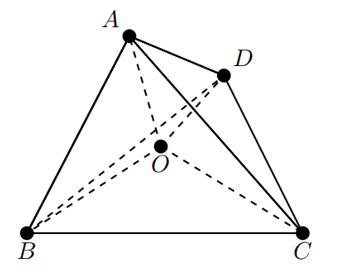
\includegraphics[width=0.32\textwidth]{assets/CMC-2025-PRE-MathA-I.png}\end{center}

\section*{CMC-2025-PRE-MathA-IV — 极小多项式与交换子}

test，L7。

设 $K$ 为数域，$A:V\to V$ 为 $n$ 维 $K$ 向量空间上的线性算子，极小与特征多项式分别为 $\mu_A,\chi_A$。定义 $\mu_{A,\alpha}$ 为使 $p(A)\alpha=0$ 的最低次首一多项式。证明：(1) 存在 $\alpha\in V$ 使 $\mu_A=\mu_{A,\alpha}$；(2) $K[A]\alpha=\{p(A)\alpha:p\in K[x]\}$ 是维数 $\deg\mu_{A,\alpha}$ 的 $A$ 不变子空间；(3) 若 $\mu_A=\chi_A$，则对任意线性算子 $B$，$AB=BA$ 当且仅当存在 $f\in K[x]$ 使 $B=f(A)$。

\section*{CMC-2025-PRE-MathA-V — 二阶导数上界与插值刚性}

test，L5。

设 $f\in C[0,1]\cap C^2(0,1)$，$\sup_{x\in(0,1)}f^{\prime\prime}(x)=2$。证明存在唯一二次多项式 $P(x)=x^2+bx+c$，满足P(0)=f(0)、P(1)=f(1)，且以下之一成立：(1) 对全部0<x<1，f(x)>P(x)；(2) 在[0,1]上f=P。

\section*{CMC-2025-PRE-MathA-VI — 自然密度上的Riemann和}

test，L7。

设 $A\subseteq\mathbb Z_{>0}$，对 $0\le a\le b\le1$ 定义 $S_n(a,b)=\#\{k\in A:an\le k\le bn\}$，且 $S_n(0,1)/n\to p$。(1) 对 $0<a<b<1$ 证明 $S_n(a,b)/n$ 收敛并求极限；(2) 对任意在 $[0,1]$ 上Riemann可积的 $f$，证明 $\lim_{n\to\infty}\frac1n\sum_{1\le k\le n,\ k\in A}f(k/n)=p\int_0^1f(x)dx$。

\section*{CMC-2025-PRE-MathB-I — 四面体重心线的交点}

test，L4。

在非退化四面体ABCD中，$e_1=\overrightarrow{AB},e_2=\overrightarrow{AC},e_3=\overrightarrow{AD}$。O1,O2,O3分别为面BCD、ACD、ABD的重心。(1) 在仿射坐标系 $(A;e_1,e_2,e_3)$ 中求O1；(2) 证明AO1、BO2、CO3共点；(3) 求该交点坐标。

\section*{CMC-2025-PRE-MathB-II — 加性唯一集的指数和}

test，L5。

设整数集合S有N个元素，N≥1。若 $n_1,n_2,n_3,n_4\in S$ 且 $n_1+n_2=n_3+n_4$，则 $n_1=n_3$ 或 $n_1=n_4$。令 $f(x)=\sum_{n\in S}e^{2\pi inx}$。(1) 求 $\int_0^1|f|^2dx$ 与 $\int_0^1|f|^4dx$；(2) 证明 $\int_0^1|f|dx\ge1/(2\sqrt N)$。

\section*{CMC-2025-PRE-MathB-III — 同时指定多个行列式}

test，L5。

设整数 $m,n>2$，$a_1,\ldots,a_{m+1}\in\mathbb Q$。证明：(1) 存在 $m$ 个有理 $n$ 阶矩阵 $B_j$ 使 $\det B_j=j$；(2) 存在 $m$ 个有理 $n$ 阶矩阵 $A_j$ 使 $\det A_j=a_j$ 且 $\det(A_1-A_2-\cdots-A_m)=a_{m+1}$。

\section*{CMC-2025-PRE-MathB-IV — 模整数的秩下界}

test，L5。

设A为n阶矩阵，主对角线元素都为3，其余元素均取2或2029。证明rank A为n或n−1。

\section*{CMC-2025-PRE-MathB-V — 方程根序列的单调极限}

test，L4。

对正整数 $k$：(1) 证明 $x^{3k+1}+x^2-6x+1=0$ 在 $(0,1/2)$ 内有唯一根 $x_k$；(2) 证明根序列严格单调；(3) 求极限。

\section*{CMC-2025-PRE-MathB-VI — 奇异微分不等式的二择一}

test，L5。

设 $f\in C^1[0,1]$，对 $0<x<1$ 有 $f(x)\ln^2x+xf^{\prime}(x)\le0$。证明以下之一成立：(1) 对所有x∈(0,1)，$\int_0^1f(t)dt<\int_0^xf(t)dt\le0$；(2) f在[0,1]恒为0。

\section*{CMC-2025-PRE-NonMathA-I-1 — Taylor主项匹配}

test，L2。

设 $f(x)=x-\ln(1+x)-\tfrac12x\sin x$，$g(x)=ax^3$，且 $\lim_{x\to0}f(x)/g(x)=1$。求a。

\section*{CMC-2025-PRE-NonMathA-I-3 — 变上限积分的四阶极限}

test，L2。

计算 $\displaystyle\lim_{x\to0}\frac{\int_0^{\sin^2x}\ln(1+t)dt}{(\sqrt[3]{1+x^3}-1)\sin x}$。

\section*{CMC-2025-PRE-NonMathA-I-5 — 球面截线的对称积分}

test，L4。

设L为球面 $x^2+y^2+z^2=4$ 与平面 $x+y+z=3$ 的交线。计算 $\displaystyle\int_L(x^2+2xy)\,ds$。

\section*{CMC-2025-PRE-NonMathA-II — 函数方程的导数积分自洽}

test，L4。

设f在实轴连续，在0可导，并满足 $f(x)=x^3+x^2\lim_{t\to0}f(t)/t-x\int_0^1f(t)dt$。求f。

\section*{CMC-2025-PRE-NonMathA-IV — 平面围成区域上的三重积分}

test，L4。

设 $\Omega$ 为平面 $x=0,x=y,y=z,z=1,z=2$ 围成的有界区域。计算 $\displaystyle\iiint_\Omega\frac{dx\,dy\,dz}{\sqrt{y^2+z^2}}$。

\section*{CMC-2025-PRE-NonMathA-V — 倍角乘积级数收敛}

test，L5。

对每个实数x，判断 $\displaystyle\sum_{n=1}^\infty a_n(x)$ 的敛散性，其中 $a_n(x)=\prod_{k=0}^n\sin^2(2^k x)$。

\section*{CMC-2025-PRE-NonMathA-VI — Wronskian条件与积分正性}

test，L7。

设 $a<b$，$f,g\in C^1[a,b]$，满足 $\int_a^bf=\int_a^bg=0$，$f^{\prime}(x)g(x)-f(x)g^{\prime}(x)>0$ 对全部 $x\in[a,b]$ 成立，且g在(a,b)恰有一零点ξ。证明：(1) $\int_a^b f(x)\int_a^xg(s)ds\,dx=-\int_a^b g(x)\int_a^xf(s)ds\,dx$；(2) 左侧积分严格大于0。

\section*{CMC-2025-PRE-NonMathB-I-1 — 局部二阶导数}

test，L2。

已知 $y=x^2e^{\sin x}$，求 $y^{\prime\prime}(0)$。

\section*{CMC-2025-PRE-NonMathB-I-2 — 空间平面方程}

test，L2。

求经过原点及 $(6,-3,2)$，且与平面 $4x-y+2z-8=0$ 垂直的平面方程。

\section*{CMC-2025-PRE-NonMathB-I-3 — 函数对称性的定积分}

test，L2。

设连续函数满足 $f(x)+f(-x)=2$。计算 $\displaystyle\int_{-1}^1(f(x)+x^2\ln(x+\sqrt{x^2+1}))dx$。

\section*{CMC-2025-PRE-NonMathB-I-4 — 复合隐函数的偏导数}

test，L2。

设 $f(u,v)$ 有一阶连续偏导，$f(2,0)=3$，$f_u(2,0)=5$。隐函数 $z=z(x,y)$ 满足 $xz=f(2x-y,xyz)$。求 $z_x(1,0)$。

\section*{CMC-2025-PRE-NonMathB-I-5 — 对数反常积分}

test，L2。

计算 $\displaystyle\int_1^{+\infty}\frac{\ln x}{(1+x)^2}dx$。

\section*{CMC-2025-PRE-NonMathB-II — 方向导数与旋转曲面面积}

test，L4。

设 $f(x,y)=ax^2+by^2+1$。在 $(4,3)$ 处的全部方向导数中，沿 $-4\mathbf i-3\mathbf j$ 的方向导数最大且为10。(1) 求a,b；(2) 求曲面 $z=f(x,y)$ 被 $z=0$ 截下的有限部分面积。

\section*{CMC-2025-PRE-NonMathB-III — 隐式曲面的局部极值}

test，L4。

求由 $2x^2+2y^2+z^2+8xz-z+8=0$ 确定的隐函数 $z=z(x,y)$ 的局部极值。

\section*{CMC-2025-PRE-NonMathB-IV — 三角代换的微分方程}

test，L4。

求微分方程 $xy^{\prime}\ln x\sin y+(1-x\cos y)\cos y=0$ 的通解。

\section*{CMC-2025-PRE-NonMathB-VI — 均值偏差的积分界}

test，L4。

设 $a<b$，$f\in C^1[a,b]$，$A=(b-a)^{-1}\int_a^bf(x)dx$。证明 $\displaystyle\int_a^b|f(x)-A|^2dx\le\frac{(a-b)^2}{2}\int_a^b|f^{\prime}(x)|^2dx$。

\end{document}
